
\chapter{Background and motivation \label{chap:Background-and-motivation}}

% First paragraph has no indentation.

\noindent Short introduction to the content of this chapter.


\section{Optimization models}

Optimization may be informally defined as the procedure of finding
better solutions to a given problem, which usually model some physical
phenomenon. In our every day life, we are constantly solving small
optimization problems, like choosing the shortest route to a friend's
house, or organizing the appointments in our agenda. In general, these
problems are small enough for us to find a good solution without extra
help, but as they become larger and more complex, the aid of computers
for their resolution is unavoidable.

Complex multidimensional optimization problems are popular in engineering,
economics, physics and other scientific fields. When solving an optimization
problem, the objective is to find a ``good'' solution in a ``reasonable''
computational time. In this respect, the field of mathematical optimization
has received a lot of attention by the scientific community during
the last decades. However, both ``good'' and ``reasonable'' are
problem, application and context-specific concepts, in which the biggest
challenge of selecting an appropiate optimization approach usually
lays.

Mathematical optimization involves the process of finding solutions
from a group of possible decisions, which may be defined as:

\begin{equation}
\min f(\vec{x})\vec{x}\in\Omega\subseteq\mathbb{R}^{n},
\end{equation}


\noindent where $\vec{x}=(x_{1},\dots,x_{n})$ is a vector representing
the decision variables, $f(\vec{x})$ is the objective function measuring
the quality of the decisions and $\Omega$ is the set of feasible
solutions of the problem, also known as search space. Note that the
objective function $f$ makes it possible to define a total order
relation between any pair of solutions in the search space $\Omega$.

The search space $\Omega$ may also be expressed as a solution to
a system of equalities or inequialities, e.g.:

\begin{eqnarray}
g(x_{1},\dots,x_{n}) & \leq & 0\nonumber \\
h(x_{1},\dots,x_{n}) & = & 0
\end{eqnarray}


Optimization problems involving the maximization of the objective
function also fall into this category, since:

\begin{equation}
\max f(\vec{x})=-\min(-f(\vec{x}))\label{eq:02-maximization_minization_problem_relation}
\end{equation}


A point $\vec{x}^{*}$ is considered to be an unrestricted local minimum
of a function $f$ if it holds a better value than all its neightbours,
i.e. there exits $\epsilon>0$ so that:

\begin{equation}
f(\vec{x}^{*})\leq f(\vec{x})\forall\vec{x}|\vec{x}-\vec{x}^{*}|<\epsilon\label{eq:02-local_minimum}
\end{equation}


Similarly, a point $\vec{x}^{*}$ is considered to be an unrestricted
global minimum of a function $f$ if it holds a better value than
all others, i.e.:

\begin{equation}
f(\vec{x}^{*})\leq f(\vec{x})\forall\vec{x}\in\mathbb{R}^{n}\label{eq:02-global_minimum}
\end{equation}


The concepts of local and global minimum are considered strict if
the inequalities of Equations \ref{eq:02-local_minimum} and \ref{eq:02-global_minimum}
are strict. 

Likewise, the definition of local and global maximum is given by the
existing relation between a minimization and a maximization problem,
as specified in Equation \ref{eq:02-maximization_minization_problem_relation},
i.e. a point $\vec{x}^{*}$ is a local or global maximum of a function
$f$ if and only if $\vec{x}^{*}$ is a local or global minimum of
function $-f$, respectively.


\subsection{Gradient-based optimization}

Gradient-descent methods are among the oldest and most studied optimization
approaches. They are based on the derivative of the optimized function,
using the first and even the second derivate of a function $f$. The
name gradient follows from the derivative of multidimensional functions,
$\nabla f(\vec{x})$, which is simply a vector where each element
is the slope of $\vec{x}$ in that dimension, i.e. $<\frac{\partial f}{\partial x_{1}},\dots,\frac{\partial f}{\partial x_{n}}>$
\cite{Luke-Essentials_of_metaheuristics:2009}.

The principle behind gradient-descent methods is rather simple. Starting
from an arbitrary value for $x$, we iteratevily add a small positive
value to it, i.e.:

\begin{equation}
x\leftarrow x-\alpha f'(x),
\end{equation}


\noindent where $\alpha$ is a small positive value. Consequently,
a positive slope will make $x$ decrease, whereas a negative slope
will make it increase. Figure \ref{fig:02-gradient_descent} shows
an example of this behaviour. Therefore, $x$ will gradually move
down the function until it finds its minimum, where $f'(x)$ is zero,
causing it to stop.

\begin{figure}
\centering

\includegraphics[width=0.4\textwidth]{02-background_and_motivation/img/optimization_cycle}

\caption{Gradient descent with a negative slope, i.e. $x$ is increasing \cite{Luke-Essentials_of_metaheuristics:2009}.
\label{fig:02-gradient_descent}}
\end{figure}


However, gradient methods have certaing drawbacks that make them unsuitable
for tackling a wide range of optimization problems. Take, for example,
the time they take to converge. As gradient descent approaches a function
minimum, it will skip this point and land on the other side. In the
next step, something similar will happen, but this time from the other
side of the minimum point, thus slowly approaching to the target in
a ``zig-zag'' way. This behavior is directly related to the slope
of the function at the given point, i.e. a steepest slope translates
into a larger jump, and may be allivieatted by adjusting the value
of $\alpha$. However, some functions (or regions of functions) may
require smaller values, while for others a bigger value would be more
appropiate. Newton's method improves this by taking the second derivative
of the function into account, i.e.:

\begin{equation}
x\leftarrow x-\alpha\frac{f'(x)}{f''(x)},
\end{equation}


\noindent thus adjusting the value of $\alpha$ as it converges towards
a point with zero slope \cite{Luke-Essentials_of_metaheuristics:2009}.

Another issue is how other points are handled. Beside maxima and minima
points, some functions also contain saddle points (known as inflection
points in one-dimensional functions). Clearly, the first derivative
of a saddle point is zero, meaning gradient descent will stop looking
for the minimum, even though it hasn't found it (see Figure ???).
Newton's method, on the other hand, does not help either. Moreover,
in this case, we would be even dividing by zero! These observations
clearly show how gradient methods get caught in local optima. We define
local optima of a function as the optima (or minima in our case) of
a local region. Similarly, global optima are defined as the optima
of the whole domain of a function. It follows that gradient methods,
as gradient descent or Newton\textquoteright{}s method, are local
optimization algorithms \cite{Luke-Essentials_of_metaheuristics:2009}.

But maybe the biggest concern with gradient-based methods is they
assume the function under optimization is derivable. This assumption
holds only when optimizing a well-formed mathematical function. Unfortunately,
this is generally not the case, since in most cases the gradient is
not computable because the function is not known. The only available
approach in such situations is creating inputs to the function in
order to assess their quality.


\subsection{Linear programming???}

\{Hace falta escribir algo sobre linear programming???\}

Generally, when dealing with real-world problems, the availability
of analytical optimization models is not guaranteed. Indeed, for some
applications, simulations or physical models are the only available
techniques to evaluate the objective function. \{Mathematical programming
and constraint programming approaches require an explicit mathematical
formulation that is impossible to derive in problems where simulation
is relevant {[}288{]} - from Talbi\}???


\subsection{Metaheuristics}

Metaheuristics, a term proposed by Glover in \cite{Glover-Future_paths_for_integer_programming_and_links_to_artificial_intelligence:1986},
represent a group of approximation algorithms designed to combine
basic heuristic principles with advanced high-level guidance methods,
targeted at improving the efficiency of a search process. These techniques
are meant to finding good solutions to a given problem, for which
the mathematical function is not available or its search space is
big enough for an exahaustive search to be unfeasible \cite{Kochenberger_Handbook_of_metaheuristics:2003}.

From the theorical point of view, metaheuristics represent a subset
of stochastic optimization, since they use some degree of randomness
to find optimal (or as optimal as possible) solutions to hard problems.
They are the most general of these kinds of algorithms, and are applied
to a wide range of problems \cite{Luke-Essentials_of_metaheuristics:2009}.

The characterization given by Blum and Roli \cite{Blum-Metaheuristics_in_combinatorial_optimization_overview_and_coconceptual_comparison:2003}
provides clear overview of the fundamental properties associated with
metaheuristics:
\begin{itemize}
\item metaheuristics are strategies that \textquotedblleft{}guide\textquotedblright{}
the search process;
\item their goal is to efficiently explore the search space in order to
find optimal or near-optimal solutions;
\item they build upon techniques which range from simple local search procedures
to complex learning processes;
\item they are approximate and usually non-deterministic;
\item they may incorporate mechanisms to avoid getting trapped in confined
areas of the search space;
\item their basic concepts permit an abstract-level description, which is
not problem-specific;
\item they may make use of domain-specific knowledge in the form of heuristics
that are controlled by the upper level strategy;
\item advanced metaheuristics use search experience (implemented as some
form of memory) to guide the search process.
\end{itemize}
The strategies used by metaheuristics should provide a dynamic balance
between the exploitation of the accumulated search experience (which
is commonly called intensification) and the exploration of the search
space (which is commonly called diversification) \cite{Blum-Metaheuristics_in_combinatorial_optimization_overview_and_coconceptual_comparison:2003}.
This balance provides the necessary means to quickly identify promising
regions, and early discarding those which have already been explored
or don't provide solutions of better quality. Promising regions within
the search space, which are identified by the obtained ``good''
solutions, are thoughfully explored during the intensification phase,
hoping to find better solutions. On the other hand, during the diversification
phase, not yet visited regions are explored, making sure the search
space as a whole is evenly explored, thus avoid confining the search
to a reduced number of regions. In this context, the ultimate search
algorithm in terms of diversification is random search. Random search
generates a random solution in the search space at each iteration,
without using memory \cite{Talbi_Metaheuristics:2009}. In terms of
intensification, iterative local search is the extreme algorithm.
The vase steepest local search algorithm selects, at each iteration,
the best neighboring solution that improves the current one \cite{Talbi_Metaheuristics:2009}.


\subsection{The feasibility problem, i.e. why fast evaluation methods are key
for successful optimization}


\subsection{The reproducibility problem}

A quick review of the state-of-the-art in 3G network optimization
indicates that software, providing good computational models, is a
very expensive tool for science. Moreover, since the vast majority
of this software is proprietary, it relies on closed source, formats
and protocols, which disclosure is explicitly forbidden by their licenses.
This fact creates a big hurdle to one of the key phases of scientific
methodology \cite{gauch2002scientific}: experimental reproducibility.


\section{Optimization of radio networks}

Once a mobile network is launched, an important part of its operation
and maintenance is monitoring the quality characteristics and changing
parameter values in order to improve its performance.

The evolution from 2G to 3G has introduced not only the technology
needed to increase both data and voice capacity, but also a greater
complexity in terms of network planning, deployment, and configuration,
which have rendered most of the traditionally used methods to be ineffective.
In a traditional approach (i.e. manual), during the network planning
and maintenance processes, a network planning software tool would
execute the analysis, while the human would make the change decisions.
Therefore, a radio planning engineer configures network parameters
manually and the network planning tool analyzes the given configuration.
If the obtained results are not acceptable, the analysis process has
to be repeated several times, until the goal is achieved.

Modern 3G radio networks are large and many of their key parameters
are interdependent. Since an engineer is not able to cope with the
level of complexity present in such systems, the computer, along with
specialized software, guides the engineer to the most appropriate
configuration for the network. In the context of this work, we will
refer to this process as optimization.

A common limitation of the implementations of such optimization methods,
generally targeting traditional computer architectures of sequential
execution, is their inability to meet the requirements needed by real-world
mobile networks, since their computational-time complexity make them
unfeasible for practical use. When analyzing big real-world networks
with thousands of users it is necessary to reduce the execution time
of the optimization processes as much as possible, so that they are
useful for practical use.

Additionally, the implementation of the framework will benefit from
valuable advances in computer science and High Performance Computing
(HPC), in order to perform faster and more reliable simulations \cite{gorder2007multicore,wen2011gpu}.

The complexity of these systems has grown even faster than their throughput
capacity, thus making it impossible to plan 3G mobile networks with
traditional methods. In this sense, an examination of colored coverage
maps in conjunction with some statistical analysis are no longer appropriate
tools for network examination. Once a mobile network is launched,
an important part of its operation and maintenance is monitoring of
quality characteristics and changing parameter values in order to
improve performance. In this sense, we may divide these tasks in two
phases: analysis and decision \cite{nawrocki2006understanding}. The
analysis phase consists of network performance analysis, which mainly
focuses on definition and collection of Key Performance Indicators
(KPIs). KPIs are quantifiable measurements, agreed to beforehand,
that reflect, in this context, network quality factors. The second
phase deals with making decisions, based on analytical results collected
in the previous phase, about the configuration of particular parameter
settings. This process (shown in Figure \ref{fig:Optimization-cycle})
is repeated until the achieved results are acceptable.

\begin{figure}
\centering

\includegraphics[width=0.4\textwidth]{02-background_and_motivation/img/optimization_cycle}

\caption{Optimization cycle for 3G mobile networks.\label{fig:Optimization-cycle}}
\end{figure}


In a traditional method approach (i.e. manual), during network planning
and optimization processes, a network planning software tool would
execute the analysis, while the human would make the decisions. Consequently,
a radio planning engineer configures network parameters manually and
the network planning tool analyzes the given configuration. If the
obtained results are not acceptable, the analysis process has to be
repeated several times, until the goal is achieved.

Modern 3G mobile networks are large and many of their key parameters
are interdependent. Since an engineer is not able to cope with the
level of complexity present in such systems, the computer, along with
specialized software, guides the engineer to the most appropriate
configuration for the network. In the context of this work, we will
refer to this process as \emph{optimization}. The results of the optimization
process are expected to provide advice%
\footnote{Some works are already focusing on complete automation of these tasks
(i.e. without human intervention).%
} regarding deployment, extension or reconfiguration tasks of a 3G
network.


\section{Overview of optimization problems for radio networks}

Although wireless networks are increasingly more sophisticated, the
need for optimization work is still far from declining. It has been
established that most 3G radio network optimization problems are NP-hard,
since computational time grows non-polynomially with the increase
of the problem size \cite{amaldi:planning.umts.base.station.location}.
Moreover, there are other reasons directly related with the evolution
of already deployed networks that greatly increase the need for optimization
methods, as described in \cite{nawrocki2006understanding}:
\begin{itemize}
\item Network performance improvement: more users covered with the same
physical infrastructure, leaving room for parameter optimization only.
\item Changes in users\textquoteright{} profile: the introduction of new
services puts additional stress on the infrastructure, requiring additional
optimization efforts.
\item Changing propagation conditions: the allocation of a higher frequency
band for UMTS compared to GSM requires deployment of more 3G sites
than in 2G networks, mostly in urban areas, thus increasing inter-cell
interference.
\end{itemize}
In this sense, network operators have shown the need to define different
optimization targets. These targets are formed by an objective function
that maps possible values of configuration parameters into a value.
Thus, each element (solution) of the solution space is assigned a
comparable value, i.e. a real number. This number represents a quality
rating of the proposed solution and it is used to compare different
solutions among each other, and ultimately select the best one. Unfortunately,
there is no definitive objective function in the field of 3G network
optimization \cite{nawrocki2006understanding}. However, it is possible
to optimize for different targets such as coverage, base station location,
etc.

In this work, we will address network optimization methods that are
performed ``off-line'', meaning that the optimization software is
not an active functioning part of the network in operation. Statistical
data about network operation is used as the input or feedback information
for different optimization targets.

This paper gives an overview of well-known optimization problems in
3G mobile networks. At the beginning of each of the following sections,
a description of an optimization problem is given, followed by a short
survey of recently proposed optimization methods. Finally, a discussion
about the introduced methods is given, before closing with some concluding
remarks.


\subsection{Optimizing base station locations}


\subsubsection{Problem formulation}

Some references \cite{minimum.set.covering.problem:1997,minimum.set.covering.problem:1998,minimum.set.covering.problem:2000}
formulate the base station location problem in terms of the minimum
set covering problem (shown in Figure \ref{fig:The-minimum-set}).
The coverage problem is defined by considering the signal level in
every test point from all base stations and requiring that at least
one level is above a fixed threshold.

\begin{figure}[H]
\centering

\begin{minipage}[c]{0.45\textwidth}%
\centering

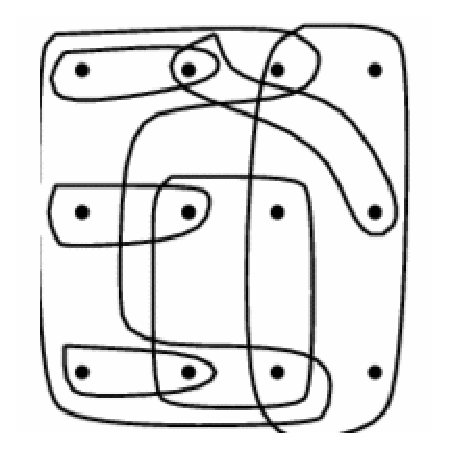
\includegraphics[width=0.6\textwidth]{02-background_and_motivation/img/set_cover_in}

(a)%
\end{minipage}\hfill{}%
\begin{minipage}[c]{0.45\textwidth}%
\centering

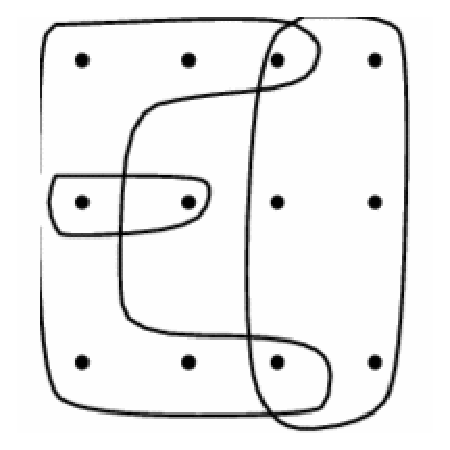
\includegraphics[width=0.6\textwidth]{02-background_and_motivation/img/set_cover_out}

(b)%
\end{minipage}\caption{The minimum set covering problem: (a) the problem input and (b) the
solution.\label{fig:The-minimum-set}}
\end{figure}


A different formulation considers the site selection problem as a
$p$-median problem, in which base station location is the only decision
variable considered. To each of the candidates solutions, an installation
cost is also associated. The $p$-median problem constitutes seeking
$p$ different locations each time, regardless of how distant the
sites are. The problem is to select one candidate site from each region
to install a base station such that the traffic capacity and the size
of the covered area are maximized with the lowest installation cost.


\subsubsection{Proposed solutions}

Aydin et al. \cite{Aydin:Heuristic.Optimization.Of.WCDMA} propose
a solution to the $p$-median problem based on three meta-heuristic
algorithms; a genetic algorithm, simulated annealing, and tabu search.
Their experimental study focuses on performance comparison between
the three algorithms.

A solution to the set covering problem is proposed by Hao et al. \cite{minimum.set.covering.problem:1997}.
A simulated annealing implementation was developed to solve the formulated
combinatorial problem. The results presented demonstrate the feasibility
of the proposed approach. Tutschku \cite{minimum.set.covering.problem:1998}
presents a specialized greedy algorithm to solve the same problem.
This work is part of the implementation of a planning tool prototype.
Mathar and Niessen \cite{minimum.set.covering.problem:2000} propose
a solution based on integer linear programming, which they claim finds
optimal solutions in most cases. They also introduce simulated annealing
as an approximate optimization technique. This approach substitutes
linear programming whenever an exact solution is out of reach because
of the complexity of the problem.

Amaldi et al. \cite{amaldi:planning.umts.base.station.location} offer
a discussion about the computational results of two different heuristics:
greedy search and tabu search. The problem formulation is based on
a set of candidate sites where the base stations can be installed,
an estimation of the traffic distribution and a propagation description
of the area to be covered. Some years later, the same authors \cite{Amaldi:Radio.planning.and.coveraga.optimization}
extended the problem formulation by also considering base station
configuration and hardware characteristics. In both works, they propose
a mixed integer programming model with which they aim to maximize
the trade-off between total traffic covered and total installation
costs. The only difference between the models is the constraint definition
of the linear program, where the constraints in \cite{amaldi:planning.umts.base.station.location}
are a subset of the constraints in \cite{Amaldi:Radio.planning.and.coveraga.optimization}.

Finally, Whitaker et al. \cite{GA.for.antenna.placement:2005} focus
on providing the required service coverage at the lowest possible
financial cost. Their framework supports the use of any multiple objective
optimization algorithm which seeks to approximate a Pareto front.
The performance of four different algorithms is explored, namely SEAMO,
SPEA2, NSGA-II and PESA.


\subsection{Optimizing antenna parameters}

There are many antenna parameters that control the coverage and interference
in the network, since the antenna shapes the emitted energy. Two important
parameters are the azimuth angle and the elevation angle (or tilt)
of the antenna. The antenna azimuth (shown in Figure \ref{fig:Antenna-azimuth})
is the direction in which the main beam of the horizontal pattern
points \cite{WCDMAforUMTS_RadioAccessForThirdGenerationMobileCommunications}.
The antenna tilt (shown in Figure \ref{fig:Antenna-tilt}) is defined
as the angle of the main beam of the antenna relative to the horizontal
plane \cite{WCDMAforUMTS_RadioAccessForThirdGenerationMobileCommunications}.
Both of these parameters have a great influence on network quality,
although antenna tilt requires less effort to implement, since most
modern radio networks already support remote electrical tilt. The
adjustment of these two parameters optimize some important aspects
of the network, namely:
\begin{itemize}
\item path loss between the base station and the mobile phone, since less
power is required for a connection, hence more power is available
for traffic; and
\item interference between neighboring cells, which leads to an overall
capacity increase.
\end{itemize}
\begin{figure}[h]
\centering

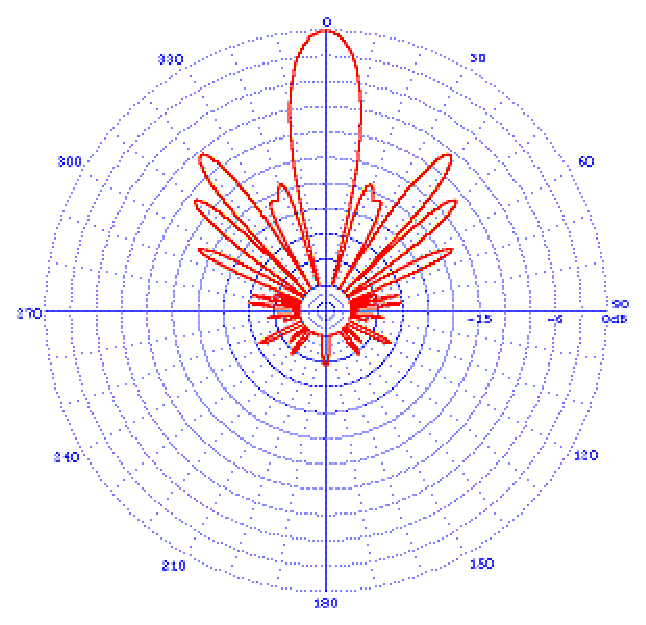
\includegraphics[width=0.3\textwidth]{02-background_and_motivation/img/azimuth}

\caption{A typical antenna azimuth pattern.\label{fig:Antenna-azimuth}}
\end{figure}


\begin{figure}
\centering

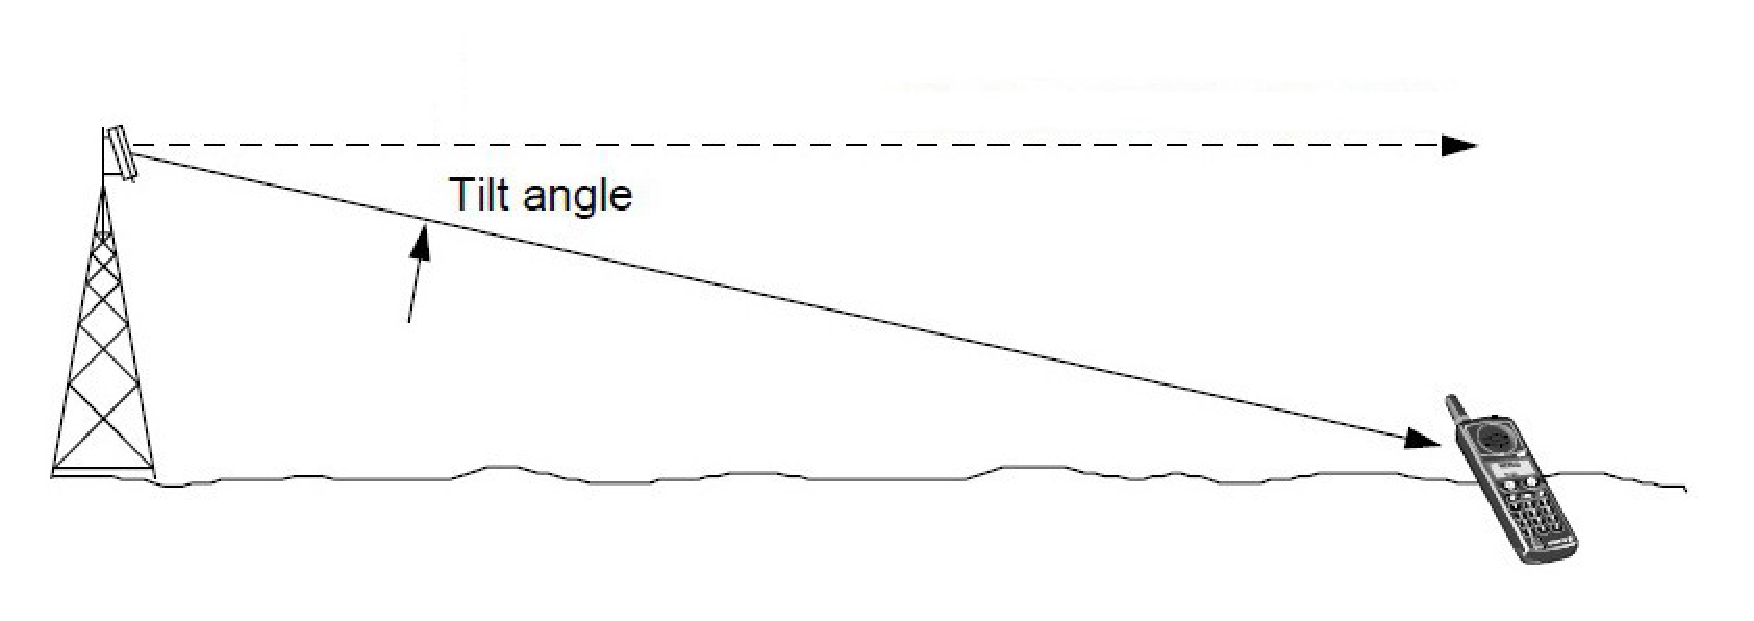
\includegraphics[width=0.6\textwidth]{02-background_and_motivation/img/tilt}

\caption{The antenna tilt angle with the horizontal plane.\label{fig:Antenna-tilt}}
\end{figure}



\subsubsection{Proposed solutions}

Karner \cite{MSc.antenna.optimization:2003} proposes an ``ad-hoc''
strategy for adjusting antenna azimuth and downtilt by analyzing the
structure of the network. The objective of this optimization is to
improve the results presented in \cite{Antenna.tilt.and.CPICH:2003}
by increasing the number of served users in the target area. In a
similar line of work, Jakl \cite{Jakl:PhD} included in his doctoral
thesis an antenna azimuth optimization algorithm, based on attempts
of avoiding coverage holes by properly adjusting the azimuth settings.

Siomina and Yuan \cite{Antenna.Configuration:2008} propose a framework
for automated optimization of antenna azimuth and tilt, including
both mechanical and electrical tilt. The implementation introduces
a simulated annealing algorithm that searches the solution space of
possible antenna configurations. The goal of the optimization is targeted
to address power sharing among cell channels and ultimately improve
High-Speed Downlink Packet Access (HSDPA) \cite{wiki:hsdpa} throughput.

Zhang et al. \cite{Antenna.azimuth.tilt:2009} present a method which
is composed of two optimization loops: the inner one and the outer
one. The inner loop concentrates on frequency planning while the outer
loop focuses on finding the optimal setting of antenna azimuth and
tilt for the current solution delivered by the inner loop. Although
frequency planning is not directly related to 3G network optimization,
we found this approach interesting enough to make a reference to it.
The inner loop could be easily replaced with some other optimization
target, e.g. common pilot channel power setting.


\subsection{Optimizing common pilot channel power}

The Common Pilot Channel (CPICH) is used as reference for handover
\cite{umts_world:handover}, cell selection \cite{3glteinfo:cellSelection},
and cell reselection \cite{flore2005:cell_reselection}. Whenever
a mobile phone is switched on, it tries to register with the cell
providing the highest received CPICH level. It also defines the effective
coverage area of the cell: according to the the CPICH power level,
the cell coverage area will enlarge or shrink. Consequently, by appropriately
adjusting the CPICH power at the base stations, the number of served
users per cell can be balanced among neighboring cells. This procedure
is called load balancing and it reduces interference, stabilizes network
operation, and facilitates radio resource management \cite{WCDMAforUMTS_RadioAccessForThirdGenerationMobileCommunications}.


\subsubsection{Proposed solutions}

Chen and Yuan \cite{CPICH.optimization:2008} optimize CPICH transmit
power starting from a uniform allocation (i.e. all cells are set with
the same transmit power level). Their objective is to enhance HSDPA
performance at cell edges while preserving control of R99 soft handover
\cite{wiki:soft_handover}. The solution approach is based on a linear-integer
mathematical model. A very similar problem and proposed solution is
presented by Siomina and Yuan \cite{CPICH.optimization:2007}. The
problem definition slightly differs from \cite{CPICH.optimization:2008}
as there is no reference to soft handover control. The solution is
also implemented as a linear program.

Olmos et al. \cite{CPICH.optimization:2003} apply simulated annealing
to the optimization of CPICH transmit powers in order to force mobile
phones to transmit to the best available cell in a service area. Their
results show decreased cell load with a consequently increased network
capacity.

Chen and Yuan \cite{CPICH.optimization:2009} present a two-phase
optimization algorithm for large-scale mobile networks. The algorithm
uses the total CPICH power consumption as a minimization objective.
The authors claim that the tabu-search-based algorithm can compute
near optimal solutions within a few seconds, even for large networks.


\subsection{Optimizing CPICH and antenna parameters}

Both the antenna tilt and azimuth directly affect the direction and
range in which the cell broadcasts its CPICH. Consequently, optimal
CPICH power is highly dependent on how the antenna tilt and azimuth
are configured at base stations. Ideal configuration of antenna tilt
and azimuth network-wise, with the objective of optimizing the CPICH
power consumption, is a challenging task. For this reason, many authors
have considered optimization methods that address all three parameters.


\subsubsection{Proposed solutions}

Varbrand et al. \cite{Coverage.optimization.on.CPICH.tilt.and.azimuth:2006}
approach the optimization of service coverage (see section \ref{sec:Optimizing-coverage})
by considering all three configuration parameters, namely: CPICH transmit
power, antenna tilt, and antenna azimuth. Their simulated annealing
algorithm searches the solution space of possible configurations in
order to find improvements in network performance and total transmitted
power. Interestingly, the algorithm is efficient enough to optimize
large networks without using excessive computing resources.

Siomina \cite{CPICH.and.antenna.tilt.optimization:2005} combines
optimization of base station antenna tilts and CPICH power to reduce
the total interference level and to improve network capacity. The
introduced algorithm optimizes the antenna downtilt setting so that
the total CPICH power in the network is minimized.

Neubauer et al. \cite{Antenna.tilt.and.CPICH:2003} present two optimization
algorithms for finding an optimal setting of antenna tilt and CPICH
power of the base stations. The first algorithm builds on a rule-based
approach, while the second one extends it by incorporating simulated
annealing. An evaluation of both techniques shows that the second
algorithm returns better results.

Jakl et al. \cite{GA.for.tilt.and.CPICH:2004} proposed a problem-specific
genetic algorithm to tackle the optimization of antenna tilts and
CPICH transmit powers. The goal of the optimization is to increase
network capacity. The implementation involves a deterministic fitness
selection scheme, a problem specific recombination operator and an
improved mutation operator. After the initial identification of the
best individuals, a local optimization technique is used to improve
their fitness.


\subsection{Optimizing coverage \label{sec:Optimizing-coverage}}

Coverage is maybe the most common optimization objective considered
in 3G network optimization. The objective function for coverage optimization
may be defined as follows:

\[
f_{cov}=\frac{A_{covered}}{A_{total}}
\]


\nomenclature[S]{$f_{cov}$}{Objective function for the coverage optimization problem.}\nomenclature[S]{$A_{covered}$}{Area, covered by the mobile network.}\nomenclature[S]{$A_{total}$}{Total area under optimization of mobile-network coverage.}

where $A_{covered}$ represents the area covered by the network and
$A_{total}$ represents the total area under optimization. Thus, the
expression $f_{cov}$ represents the portion of the total area that
is actually under network coverage. This value ranges from 0 (no coverage)
to 1 (total coverage).

The area being optimized is usually divided in squares (or pixels)
of a certain size, which may vary from 10 to 100 meters, creating
a grid of a certain resolution. A square is considered covered, if
the signal to noise ratio is above a given threshold \cite{3GPP_TS_25.133}.
It is also common to use a test function $cov(x,y)$\nomenclature[S]{$cov(x,y)$}{Returns 1 if the coordinate $(x,y)$ is under mobile-network coverage.},
which returns 1 if the square located at $(x,y)$ is covered, and
0 otherwise.


\subsubsection{Proposed solutions}

Siomina and Yuan \cite{Siomina:Minimum.pilot.power.for.service.coverage}
consider the problem of minimizing pilot power subject to the coverage
constraint. Their approach consists of mathematical programming models
and methods, based on a linear-integer mathematical formulation of
the problem. A special numerical analysis studies the trade-off between
service coverage and pilot power consumption for different test networks.

Capone et al. \cite{Amaldi:Radio.planning.and.coveraga.optimization}
investigate mathematical programming models for supporting decisions
on where to install new base stations and how to select their configuration
(antenna height and tilt, sector orientations, maximum emission power,
pilot signal, etc.) so to find a trade-off between maximizing coverage
and minimizing costs. The overall model takes into account signal-quality
constraints in both uplink and downlink directions, as well as the
power control mechanism and the CPICH signal.

Valkealahti et al. \cite{Coverage.balance:2002} propose a method
for automatic setting of CPICH power. The control algorithm applies
total transmission power measurements from the base station, neighboring
cells and mobile terminals to determine the pilot qualification. The
CPICH power is then periodically updated based on a group of heuristic
rules in order to improve coverage and load balance. A similar approach
is described by Parkinnen et al. \cite{Coverage.optimization.with.cost.function:2002}
where some network performance parameters are combined with service
coverage in a cost function. The pilot power of a cell is periodically
updated with a gradient descent method that minimizes the afore mentioned
function.


\subsection{Optimizing alignment of soft-handover areas}

We have defined this new problem. About the connecting of this 3G-specific
problem with LTE ...???


\subsection{Discussion}

In the field of 3G network optimization, comparing the efficiency
of different optimization methods has proven to be a very difficult
task. There are several reasons for this, among which we have identified
the following:
\begin{itemize}
\item The networks on which the experiments are carried out are not standardized.
Thus, it is problematic to set up an environment in which the presented
results may be reproduced.
\item There are no ``open'' implementations of 3G mobile network simulators.
On the contrary, there is a vast variety of proprietary (or ``closed'')
network simulators that only increase the ambiguity regarding the
experimental environment used for a certain network layout and configuration.
Moreover, some of the ``closed'' network simulators do not even
account on the built-in path loss estimation methods used.
\item Only a small part of the referenced optimization methods perform their
experiments on real-life networks, that have been already deployed
and are currently running. This fact creates a gap between the research
field and the industry (i.e. the application area) and it is counterproductive
for both the researchers and the network operators, since they don't
benefit from mutual collaboration.
\end{itemize}
We believe that the creation of a standardized framework would be
a great benefit in the field of 3G network optimization, as it would
allow researchers to compare different methods, results and solutions
in an easy, fast and objective manner. An effort in this direction
is the MOMENTUM project \cite{Momentum.project}. It was created with
the objective of setting up a standardized experimental environment
that would facilitate research cooperation and would ultimately benefit
from an improvement on the research field of 3G networks. The project
includes complete data about the terrain, properties of the service
area and hardware used in three different mobile networks. It offers
the researcher detailed information about real-life networks based
in Berlin, Lisbon and The Hague. As part of the package, there is
also a Java application programming interface (API) that eases the
implementation of some conventional tasks such as data parsing. The
main focus of project is on data, thus there is no network simulator
included. In any case, the researcher benefits from several included
traffic snapshots that help assessing different network configuration
settings. There have been no updates in the MOMENTUM project since
2005, when the last data corrections were introduced \cite{Momentum.project}.

In the context of this survey and after reviewing many different papers
on 3G network optimization, we can say that the MOMENTUM project has
not been widely adopted by the scientific community. Moreover, several
of the reviewed works do not offer detailed instructions on how to
resemble the experimental environment. Consequently, it is very complicated
(if not even impossible) to reproduce the presented results. Therefore,
the selection of optimization methods, based on the results presented
by their corresponding authors, is virtually meaningless, since the
results are not comparable with each other. For this reason, we have
decided to concentrate the following discussion on the optimization
methods used, leaving the results aside.


\subsection{Discussion about the presented methods}

Regarding the optimizations methods presented in previous chapters,
three distinctive groups emerge: genetic algorithms, linear programming
and other search methods.
\begin{description}
\item [{Genetic~algorithms}] These algorithms work on a population of
solutions that allows a more comprehensive search for optimal solutions.
As a direct consequence, an increase in running time is commonly observed.
The implementation effort of genetic algorithms is to some degree
higher than for simpler search methods (e.g. local search), but their
inherent structure greatly simplifies possible parallel implementations
and execution.
\item [{Linear~programming}] Linear optimization problems are widely used
in different optimization areas and there are many good software packages
to solve such problems. Consequently, if a problem can be modeled
as a continuous linear problem, there is usually no difficulty in
finding optimality. In the context of this survey, linear programming
has proven useful for coverage optimization in early network planning
stages.\\

\item [{Other~search~methods}] Other search methods%
\footnote{Namely, local search, simulated annealing and tabu search in the context
of this survey.%
} usually represent a compromise between running time and quality of
results. They rely on evaluating a great number of alternative configurations.
The number of parameters taken into account, as well as the evaluation
precision, directly influence their running time. These methods don't
excel in full simulation scenarios. On the other hand, some search
methods (e.g. tabu search) have powerful mechanisms to escape local
minima.
\end{description}
A short comparison of the optimization methods presented in this survey
is shown in Table \ref{tab:Comparison-of-optimization-methods}. The
comparison variables arise from the context in which the methods were
presented.

\begin{table}
\centering{\footnotesize \caption{A comparison among the presented optimization methods.\label{tab:Comparison-of-optimization-methods}}
}{\footnotesize \par}

{\footnotesize }%
\begin{tabular}{|c|c|c|}
\hline 
{\footnotesize Algorithm} & {\footnotesize Running time} & {\footnotesize Typical application}\tabularnewline
\hline 
\hline 
{\footnotesize Local search} & {\footnotesize Shorter} & {\footnotesize Solution quality improvement.}\tabularnewline
\hline 
{\footnotesize Tabu search} & {\footnotesize Shorter} & {\footnotesize Solution quality improvement.}\tabularnewline
\hline 
{\footnotesize Simulated annealing} & {\footnotesize Longer} & {\footnotesize Initial search of the solution space.}\tabularnewline
\hline 
{\footnotesize Genetic algorithm} & {\footnotesize Longer} & {\footnotesize Initial search of the solution space and solution quality
improvement.}\tabularnewline
\hline 
{\footnotesize Linear programming} & {\footnotesize (formulation dependent)} & {\footnotesize Coverage network planning.}\tabularnewline
\hline 
\end{tabular}
\end{table}



\section*{Summary}

The variety of optimization problems that have been introduced in
the previous sections differ in many aspects like implementation,
running time and solution quality. Picking the right method for a
given situation depends on the optimization task and the desired results.
Since computation time is usually an important restriction, simpler
and faster methods may be preferable. 

Beside the convenience of a survey such as the one presented in this
work, it is very important to develop a feeling for the properties,
advantages and drawbacks of the respective methods. Moreover, radio
expert's recommendations regarding solution interpretation and feedback
from everyday network operation, are an essential input for creating
quality optimization methods. In this sense, and based on our own
experience, the expert's advice is irreplaceable and a most valuable
contribution to the research work.

Also, as it may be observed in some of the presented references, it
is often advisable to combine different methods. Therefore, a simple
optimization method may find a subset of reasonable parameter configuration,
whereas a more complex method could be applied afterward, to refine
the search. Sometimes it may also be useful to apply a simple search
method at the end to find better solutions in the vicinity of a current
promising one.
